\documentclass[emulatestandardclasses]{scrartcl}
\usepackage{graphicx}
\usepackage{color}
\usepackage[ngerman]{babel}
\usepackage{hyperref}
\usepackage{fullpage}
\usepackage[dvipsnames]{xcolor}
\usepackage{calc} 
\usepackage{enumitem}
\usepackage{titlesec}
\newcommand{\todo}[1]{\textcolor{red}{TODO: #1}\PackageWarning{TODO:}{#1!}}
\date{\vspace{-3ex}}
\begin{document}

\title{
	\includegraphics*[width=0.75\textwidth]{ErstesSem/images/hu_logo.png}\\
	\vspace{24pt}
	Kritische Theorie der Gesellschaft: Horkheimer und Adorno}
\subtitle{Proseminar SS 17\\
          Dr. Arnd Pollmann\\
          Philosophisches Institut I \\ 
          Humboldt Universit"at zu Berlin}
\author{Lennard Wolf\\
        \small{\href{mailto:lennard.wolf@student.hu-berlin.de}{lennard.wolf@student.hu-berlin.de}}}
\maketitle
\begin{abstract}

In den 1930er-Jahren ist rund um das Institut f"ur Sozialforschung in Frankfurt a.M. ein sozialkritischer und zeitdiagnostischer Forschungszusammenhang entstanden, den man "`Kritische Theorie"' oder auch "`Frankfurter Schule"' nennt. Unter der Schirmherrschaft der Philosophie wurden dort interdisziplin"are Forschungsvorhaben durchgef"uhrt, die im Anschluss an Karl Marx und Sigmund Freud vor allem der zentralen Frage nachgehen sollten, warum in Deutschland, trotz enorm wachsender sozialer Probleme, die sozialistische Revolution ausgeblieben war. Als Gr"undungsv"ater der Frankfurter Schule gelten Max Horkheimer und Theodor W. Adorno. Im Seminar werden wir eine Auswahl ihrer wichtigsten Arbeiten diskutieren. Die beiden Denker haben sich als au"serordentlich einflussreich erwiesen und die Studentenbewegung von 1968 ebenso gepr"agt wie das Denken nachfolgender Generationen kritischer Sozialphilosoph\_innen im Frankfurter "`Raum"' (z.B. J"urgen Habermas oder Axel Honneth).

\end{abstract}
\newpage

\tableofcontents
\listoffigures
\newpage


\section{Einf"uhrung / Adorno: Minima Moralia, Nr. 18
\\(19.04.17)}

\subsection{Einf"uhrung}

\begin{itemize}
  \item Entfremdetes Wohnen, maschinisierung des Wohnens $\rightarrow$ Selbes Denken das zu den KZs gef"uhrt hat
  \item Es gibt kein richtiges Leben im Falschen
\end{itemize}

\subsection{Adorno: Minima Moralia, Nr. 18 ("`Asyl f"ur Obdachlose"')}



\section{Horkheimer: "`Zur Kritik der gegenw"artigen Gesellschaft"'
\\(26.04.17)}

\subsection{Lekt"urenotizen}

\begin{description}[leftmargin=!,labelwidth=\widthof{\bfseries Dialektischer Materialismus}]
  \item[Produktivkr"afte] \emph{Alle} Kr"afte des Menschen, denen er sich bedient, um die Natur zu beherrschen (vor allem Wissenschaft, Technik)
  \item[Produktionsverh"altnisse] Beziehungen zwischen den Menschen, bestimmt durch die Produktivkr"afte 
  \item[Dialektik] ?
  \item[Dialektischer Materialismus] Durch Produktionsverh"altnisse bestimmte "Anderung der Produktivkr"afte $\rightarrow$ "Anderung der Produktionsverh"altnisse
\end{description}

\begin{itemize}
  \item Wie ist "`Kritik"' zu verstehen? Von wo kommt sie? Problem einer Kritik: Die Gesellschaft ist so "uberw"altigend f"ur den einzelnen, dass Kritik nichts mehr "andern kann $\rightarrow$ R"uckgang des Einzelsubjekts
  \item Revolution nach Marx: Unterdr"uckte Masse "uberwirft unterdr"uckende Minderheit aufgrund der immer schlechter werdenden Verh"altnisse $\rightarrow$ Heute: Staatliche Reglementierung macht, dass Bedingungen nicht zu schlecht werden | Wirtschaftliche Regulierung also nicht zum Schutze der Menschen, sondern zum Schutze der Verh"altnisse
   \item Elend ist heute anders als bei Marx: Zwar wird nicht mehr verhungert, aber man ist gefangen in Zustand und die Autonomie ist genommen
  \item Zuk"unftiges Problem: automatisierte Gesellschaft ohne h"ohere Ziele $\rightarrow$ Geist, Phantasie, Autonomie sind bedroht

\end{itemize}


\begin{enumerate}
  \item {\color{NavyBlue}Wie f"ugt sich der vorliegende Text in den thematischen Gesamtzusammenhang des Seminars ein?}\\
{\color{ForestGreen} Letzte Sitzung bei Asyl f"ur Obdachlose: Harsche Kritik an moderner Kultur anhand des Beispiels des Wohnens. Kamen zum Schluss auf die Frage: Kann Kritik ge"ubt werden ohne eine alternative anzubieten? // Text steht am ende der Frankfurter Schule. Konkreter Text da bestimmte Gegebenheit analysiert werden. Ankn"upfungspunkt zu der Frage "`Muss man wenn man kritisiert eine bessere L"osung kennen?"' die aufkam, weil Adorno nur sagt was/dass schlecht ist.}
  \item {\color{NavyBlue}Wie lautet die zentrale philosophische Frage, auf die der Text eine Antwort zu geben versucht?}\\
{\color{ForestGreen} "`Wie m"ussen wir Gesellschaftskritik verstehen"' Kritik: r"ucksichtsloses in dem Sinne dass...}
    \item {\color{NavyBlue} Wie genau lautet die Antwort, die der Text auf die soeben identifizierte Hauptfrage zu geben versucht?}\\
{\color{ForestGreen} Zu kl"aren.}
    \item {\color{NavyBlue} Welches sind die f"ur das Verst"andnis des vorliegenden Textes zentralen Begriffe und Unterscheidungen?}\\
{\color{ForestGreen} Zu kl"aren.}
    \item {\color{NavyBlue} Wie lautet in aller K"urze das im Text pr"asentierte Gesamtargument?}\\
{\color{ForestGreen} Zu kl"aren.}
    \item {\color{NavyBlue} Wie unterscheidet sich die Theorie der Inauguraldissertation
eigentlich von der in der Kritik der reinen Vernunft (1781), wenn doch beide TI beinhalten?}\\
{\color{ForestGreen} Zu kl"aren.}
\end{enumerate}


\section{Adorno: "`Gesellschaft"'
\\(10.05.17)}

\subsection{Vortrag}

\begin{itemize}
  \item Theorie der Gesellschaft kann diese nicht nur als Prozess verstehen
  \item Ges. stellt ein verh"altnism"a"siges "Ubergewicht dar, das die Individuen "uberstimmt
  \item Ges. soll f"ur uns sein, doch arbeitet auch gegen uns
  \item Gesellschaft als Begriff geht nur in der kapitalistischen Zeit
  \item Handel ist "uberall, und der Antagonismus im Handel ist die ungleiche Verteilung der Werte von Arbeit und damit eingetauschtem Kapital
\end{itemize}

\section{Adorno \& Horkheimer: "`Dialektik er Aufkl"arung"'
\\(31.05.17)}

\begin{itemize}
  \item Aufkl"arung soll Befreiung bringen, schl"agt aber um in deue Unfreiheiten
\end{itemize}


\section{VL Sozialphilosophie der Gegenwart 6 -- Sinnverlust und Gewalt\\01.06.17}

\subsection{Einf"uhrung}

\begin{itemize}
  \item Spiegel Interview mit Adorno nach dem Busenattentat
  \item Verroht die Gesellschaft immer mehr oder tr"ugt der Schein? Potenzielle Gesetze gegen Hate Speech etc. scheinen das anzudeuten..?
  \item Kritische Theorie: Interdisziplin"ares Projekt zur Erforschung der Frage, wie es der Herrschaft gelingt, die Revolution zu ersticken
  \item Zeitdiagnose: Kriege und Totalitarismus sind nicht Ausdruck historischer "`"Unvernunft"', sondern letzte Konsequenz instrumenteller Rationalit"at
  \item Hat der Hass auf der Stra"se und im Netz etwas mit de Aufkl"arung zu tun?
  \item Goya: Der Traum der Vernunft gebiert Ungeheuer (Bild einf"ugen)
  \item Herr die Not ist gro"s! Die ich rief, die Geister werd ich nun ich los (Zauberlehrling)
  \item $\rightarrow$ Ausgeburten der Vernunft/Aufkl"arung
  \item $\rightarrow$ Wir setzen dauernd Dinge in die Welt, die gr"o"ser sind als wir selbst und die wir nicht verstehen.
  \item destruktive Orientierungsnot trotz gro"ser "`Fortschritte"'
  \item \textbf{Hinterl"asst die Aufkl"arung eine metaphysische L"ucke?}
  \item Ist die Gewalt eine \emph{Ausgeburt} der Aufkl"arung und kein \emph{R"uckfall} in die Barabarei?
  \item "`Dialektik er Aufkl"arung"' wurde geschrieben inmitten einer weltpolitischen Katastrophe (WWII), in der die westliche Aufkl"arung nicht gerade den historischen Endsieg davon zu tragen scheint
  \item $\rightarrow$ vielmehr kulminieren Unvernunft, Unfreiheit, Unmenschlichkeit, Terror, Tyrannei etc. $\rightarrow$ "`neue Form der Barbarei"'?
\end{itemize}


\subsection{Das Problem des Sinnverlusts}

\begin{itemize}
  \item Das "`\emph{Sapere Aude!}"' der Aufkl"arung setzt zwei diametrale Denkbewegungen in Gang:
  \item (1) Den aufgekl"arten, engagierten, emanzipativen Einsatz f"ur einen autonomen Vernunftgebrauch (zielt auf normative Hnsicht auf Freiheit, Menschenrechte etc. ab)
  \item (2) Einen sich lebensweltlich ausbreitenden "`Kritischen Rationalismus"' und Skeptizismus
  \item $\Rightarrow$ Massive Spannung \emph{innerhalb} des "`unvollendeten Projekts"' der Aufkl"arung (Habermas)
  \item Man kann nicht zugleich ein selbstbewusstes Pl"adoyer f"ur Vernunft, Demokratie etc. abgeben \emph{UND} sich skeptisch weigern, eine jeweils bestimmte Gewissheit als f"ur alle Menschen gleicherma"sen verbindlich zu akzeptieren
  \item Verdacht: Zweite Denkbewegung (der Relativismus) tr"agt derzeit den Sieg davon ("`Postmoderne Beliebigkeit"')
  \item Wer tolerant und aufgeschlossen gegen"uber jeder noch so verwerflichen Meinung ist, verliert am Ende jedes kritische Differenzierungsverm"ogen
  \item Aufl"osung von Gewissheiten f"uhrt nicht nur zu lebenspraktischer Unsicherheit, sondern h"aufig auch zu einer sp"atmodernen "`Leere"'
  \item "`Auf dem Weg zur neuzeitlichen Wissenschaft leisten die Menscen auf Sinn Versicht"' (DdA)
  \item $\rightarrow$ Tradierte Sinnangebote werden vernichtet
  \item Sp"atmoderne Sinnsuche wird zu einem "`Privatvergn"ugen"', das sich als erm"udend und beschwerlich, sowie aussichtslos herausstellt $\rightarrow$ Nihilismus, Entzauberung der Welt
  \item "`Die zunehmende Intellektualisierung und Rationalisierung bedeutet also nicht eine zunehmende allgemeine Kenntnis der Lebensbedingungen, unter denen man steht. Sondern sie bedeutet etwas anderes: das Wissen davon oder den Glauben daran: daß man, wenn man nur wollte, es jederzeit erfahren k"onnte, da"s es also prinzipiell keine geheimnisvollen unberechenbaren M"achte gebe, die da hineinspielen, daß man vielmehr alle Dinge – im Prinzip – durch Berechnen beherrschen k"onne. Das aber bedeutet: die Entzauberung der Welt. Nicht mehr, wie der Wilde, f"ur den es solche M"achte gab, muss man zu magischen Mitteln greifen, um die Geister zu beherrschen oder zu erbitten. Sondern technische Mittel und Berechnung leisten das. Dies vor allem bedeutet die Intellektualisierung als solche."' -- Max Weber (Wissenschaft als Beruf)
  \item "`Ein Kulturmensch aber, hineingestellt in die fortw"ahrende Anreicherung der Zivilisation mit Gedanken, Wissen, Problemen, der kann 'lebensm"ude' werden, aber nicht: lebensges"attigt. Denn er erhascht von dem, was das Leben des Geistes stets neu gebiert, ja nur den winzigsten Teil, und immer nur etwas Vorl"aufiges, nichts Endg"ultiges, und deshalb ist der Tod für ihn eine sinnlose Begebenheit. Und weil der Tod sinnlos ist, ist es auch das Kulturleben als solches, welches ja eben durch seine sinnlose »Fortschrittlichkeit« den Tod zur Sinnlosigkeit stempelt."'  -- Max Weber (Wissenschaft als Beruf)
\end{itemize}

\subsection{Das Problem der Gewalt}

\begin{itemize}
  \item Die neue Lebensm"udigkeit: "`Ich schie"se, also bin ich."'
  \item "`Nur solches Denken ist hart genug, die Mythen zu zerbrechen, das sich selbst Gewalt antut."' (DdA)
  \item $\rightarrow$ wir wollen dem Leben "`neuen"' Sinn geben (neue Politik der \emph{Drastik}, die wieder unterteilt in Gut und B"ose)
  \item Allt"agliche Gewaltbereitschaft ist kein Ergbenis des Verlusts der Werte, sondern einer srastischen "`Umwertung der Werte"'
  \item Fundamentalismen reagieren auf nihilistische Unsicherheiten, indem sie klare Feindbilder und neue Orientierung/Sinn stiften
  \item Die offene Sinnfrage wird durch die Bereitschaft zur Selbstaufgabe im extremistischen "`Wir"' beantwortet
  \item Islamisus: B"ose ist die moderne Welt der Gottlosen, gut der kommende Gottesstaat
  \item $\rightarrow$ Es ist irref"uhrend, der Islam m"usse "`aufgekl"art"' werden (Trotzterror $\rightarrow$  Aufkl"arung nicht m"oglich?)
  \item Politische Jugendbewegungen: Gewaltsame Delegitimisierung der herrschenden Verh"altnisse (Islamisus, Neonazis, Linksradikale; \emph{angry white men}) $\rightarrow$  Bek"ampfung von metaphysischen Defiziten, kein Kampf f"ur die Gerechtigkeit
\end{itemize}

\subsubsection{Einw"ande}

\begin{itemize}
  \item Einwand 1: Ist Gewalt nicht blo"s die Frustration gesellschaftlich Zu-Kurz-Gekommener?
  \item $\rightarrow$ KT: ja man wertet sie auf, aber dadurch beginnt man erst sie ernst zu nehmen. Nicht blo"s Problem der sozialen Gerechtigkeit!
  \item Einwand 2: F<lie"sender "Ubergang von allt"aglicher Gewalt zu Dschihadismus?
  \item $\rightarrow$ KT: Ja!
  \item Einwand 3: Historische Kontinuit"at von faschistischer Gewalt und modernen Jugendkulturen ist "ubertrieben!
  \item $\rightarrow$ KT: nicht historsich, sondern \emph{gemeinsame Erfahrungswelt} der Gewaltt"ater
  \item Einwand 4: Kann Sinnverlust nicht auch zu Passivit"at etc. f"uhren?
  \item $\rightarrow$ KT: Ja, es gibt viele Reaktionsmuster.
  \item Einwand 5: Wurzel der Gewalt ist nicht Sinnverlust, sondern fehlende Empathie- und Bindungsf"ahigkeit!
  \item $\rightarrow$ KT: Fehlende Empathie- und Bindungsf"ahigkeit und Gewalt haben dieselbe Wurzel: instrumentelle Rationalit"at des Prinzips der "`Naturbeherrschung"'
  \item Einwand 6: Sieht die Kritische Theorie nicht 
  \item Nichts ist negativer als das st"andige Gerede von der Positivit"at, von der der 
\end{itemize}

\subsection{Diskussion}

\begin{itemize}
  \item Warum gerade M"anner, die die Gewalt ver"uben? 
  \item Sinnverlust als \emph{einzigen} Grund der dschihadistischen Bewegungen? Nein!
  \item Wenn wir die Welt nicht richtig sehen, dann \emph{gucken} wir nur nicht richtig $\rightarrow$ Das Denken ist nur verstellt, objektiv ist alles da
  \item Das egoistische Individuum ist ein direktes Produkt der Aufkl"arung
  \item Die private Gl"uckssuche ist vergebens.
\end{itemize}


\section{Foucault
\\(15.06.17)}

\subsection{Sp"atmoderne Probleme}

\begin{itemize}
  \item Arbeiterkinder werden keine Akademiker
  \item Burn-out Erkrankungen nehmen zu
  \item "`Zwang zur Selbstverwirklichung"'
  \item Unbewusste Anpassung an Systemzw"ange
  \item "Uberwachungsstaat?
  \item Kulturelle Hintergr"unde f"ur (sexualisierte) Gewaltbereichtschaft?
\end{itemize}

$\rightarrow$ Was haben diese Probleme gemein?

"`\emph{Der Mensch ist frei geboren und "uberall befindet er sich in Ketten.}"' (Rousseau)

$\rightarrow$ Autonomie oder "`stahlhartes Geh"ause der H"origkeit"' (Max Weber)?

$\rightarrow$ "`Subjekt"' vs. "`Struktur"'

\subsection{Das Problem des Subjekts}

\subsubsection{Kopernikanische Wende}

\begin{itemize}
  \item Neuzeitliche Philosophie nimmt Ausgang vom "`denkenden Subjekt"' statt vom "`objektiven Sein"' $\rightarrow$ Dualismus von Subjekt und Objekten
  \item Kopernikanische Wende: Wir "`machen"' uns die Welt
  \item Modernes Subjekt-Sein = "`selbstm"achtig"' sein
\end{itemize}

\subsubsection{Freud: "`Kr"ankungen"' des modernen Subjekts}

\begin{itemize}
  \item Empirische Wissenschaften stellen das subjekt in Frage: 
  \item $\rightarrow$ Physik zeigt Mensch ist nicht der Mittelpunkt
  \item $\rightarrow$ Biologie hebt Grenzen zwischen Mensch und Tier auf
  \item $\rightarrow$  Psychoanalyse zeigt, "`da"s das Ich nicht Herr sei in seinem eigenen Haus."' (Freud)
\end{itemize}

\subsubsection{Ist das Subjekt "`vorstrukturiert"'?}

\begin{itemize}
  \item Moderne Subjektkritik beschreibt das Subjekt als Produkt innerer und "au"serer Strukturen
  \item Das Subjekt ist nicht \emph{gegeben}, sondern \emph{gemacht}.
  \item Die jeweils vorhandenen Strukturen sind vielmehr Bedingungen f"Ur die Entstehung freier Subjektivit"at.
\end{itemize}

\subsection{Das Problem der Strukturen}

\subsubsection{Kontext}

\begin{itemize}
  \item "`Foucault als Sozialphilosoph des Poststrukturalismus."'
  \item Saussure und linguistischer Strukturalismus
\end{itemize}

\subsubsection{Foucault}

Dreidimensionale "`Genealogie"' der modernen Subjektivit"at

$\rightarrow$ "`Wie ist das moderne Subjekt das geworden, was es heute ist?"'

\begin{enumerate}
  \item "`Diskurse"': Subjektkonstitution durch Techniken der Wahrheitsproduktion (Humanwissenschaften)
  \item "`Macht"': Soziale Abrichtung durch Disziplinaranstalten (Schule, Kaserne, Gef"angnis, Psychiatrie)
  \item "`Ethik"': Selbstdisziplinierung durch Techniken der Selbstsorge (Briefe, Beichte, Tageb"ucher, Sexualit"at)
\end{enumerate}

$\rightarrow$ Beweist seltsamen Zucht- und Dressurcharakter moderner Subjektivit"at

\begin{itemize}
  \item Das Subjekt ist ein Effekt der Disposiive Diskurs/Macht/Ethik
  \item Das moderne Subjekt ist weniger frei als vielmehr "`unterworfen"' (lat. \emph{subiectum})
  \item Der Zwang ist nicht durch Gewalt erreicht.
  \item $\rightarrow$ Panoptikum als \emph{das} Paradigma der Moderne
  \item $\rightarrow$ Konstantes Gef"uhl des Betrachtetwerdens (s"akularisierte Version des "`Gott sieht alles"')
\end{itemize}

$\rightarrow$ "`Poststrukturalismus"': Die Strukturen k"onnen ver"andert werden durch Subversion.

\begin{itemize}
  \item Macht ist "`produktiv"', sie macht uns zu Subjekten und verleitet uns zum Handeln $\rightarrow$ Ohne strukturelle Zw"ange g"abe es keine nach Freiheit strebenden Subjekte
  \item $\rightarrow$ Bewusstwerdung der eigenen Verlustgeschichte des modernen Subjekts soll dessen geschw"achte Widerstandskr"afte st"arken.
  \item $\rightarrow$ Kritik an den Machtstrukturen dient zur Entwicklung freierer Verh"altnisse
\end{itemize}

\subsubsection{Einw"ande}

\begin{itemize}
  \item Einwand 1: Kritik ist "uberall sp"urbar in seinen Texten
  \item $\rightarrow$ F: ?
  \item Einwand 2: Aber warum kein Normatives Moment in seinen Texten?
  \item $\rightarrow$ F: Befreiung ist keine Frage theoretischen Expertises, sondern politischen Kampfes
\end{itemize}

Das moderne Subjekt ist ganz etwas anderes als jenes im deutschen Idealismus.

\subsubsection{Diskussion}



\newpage


%\begin{figure}[h]
%	\centering
%	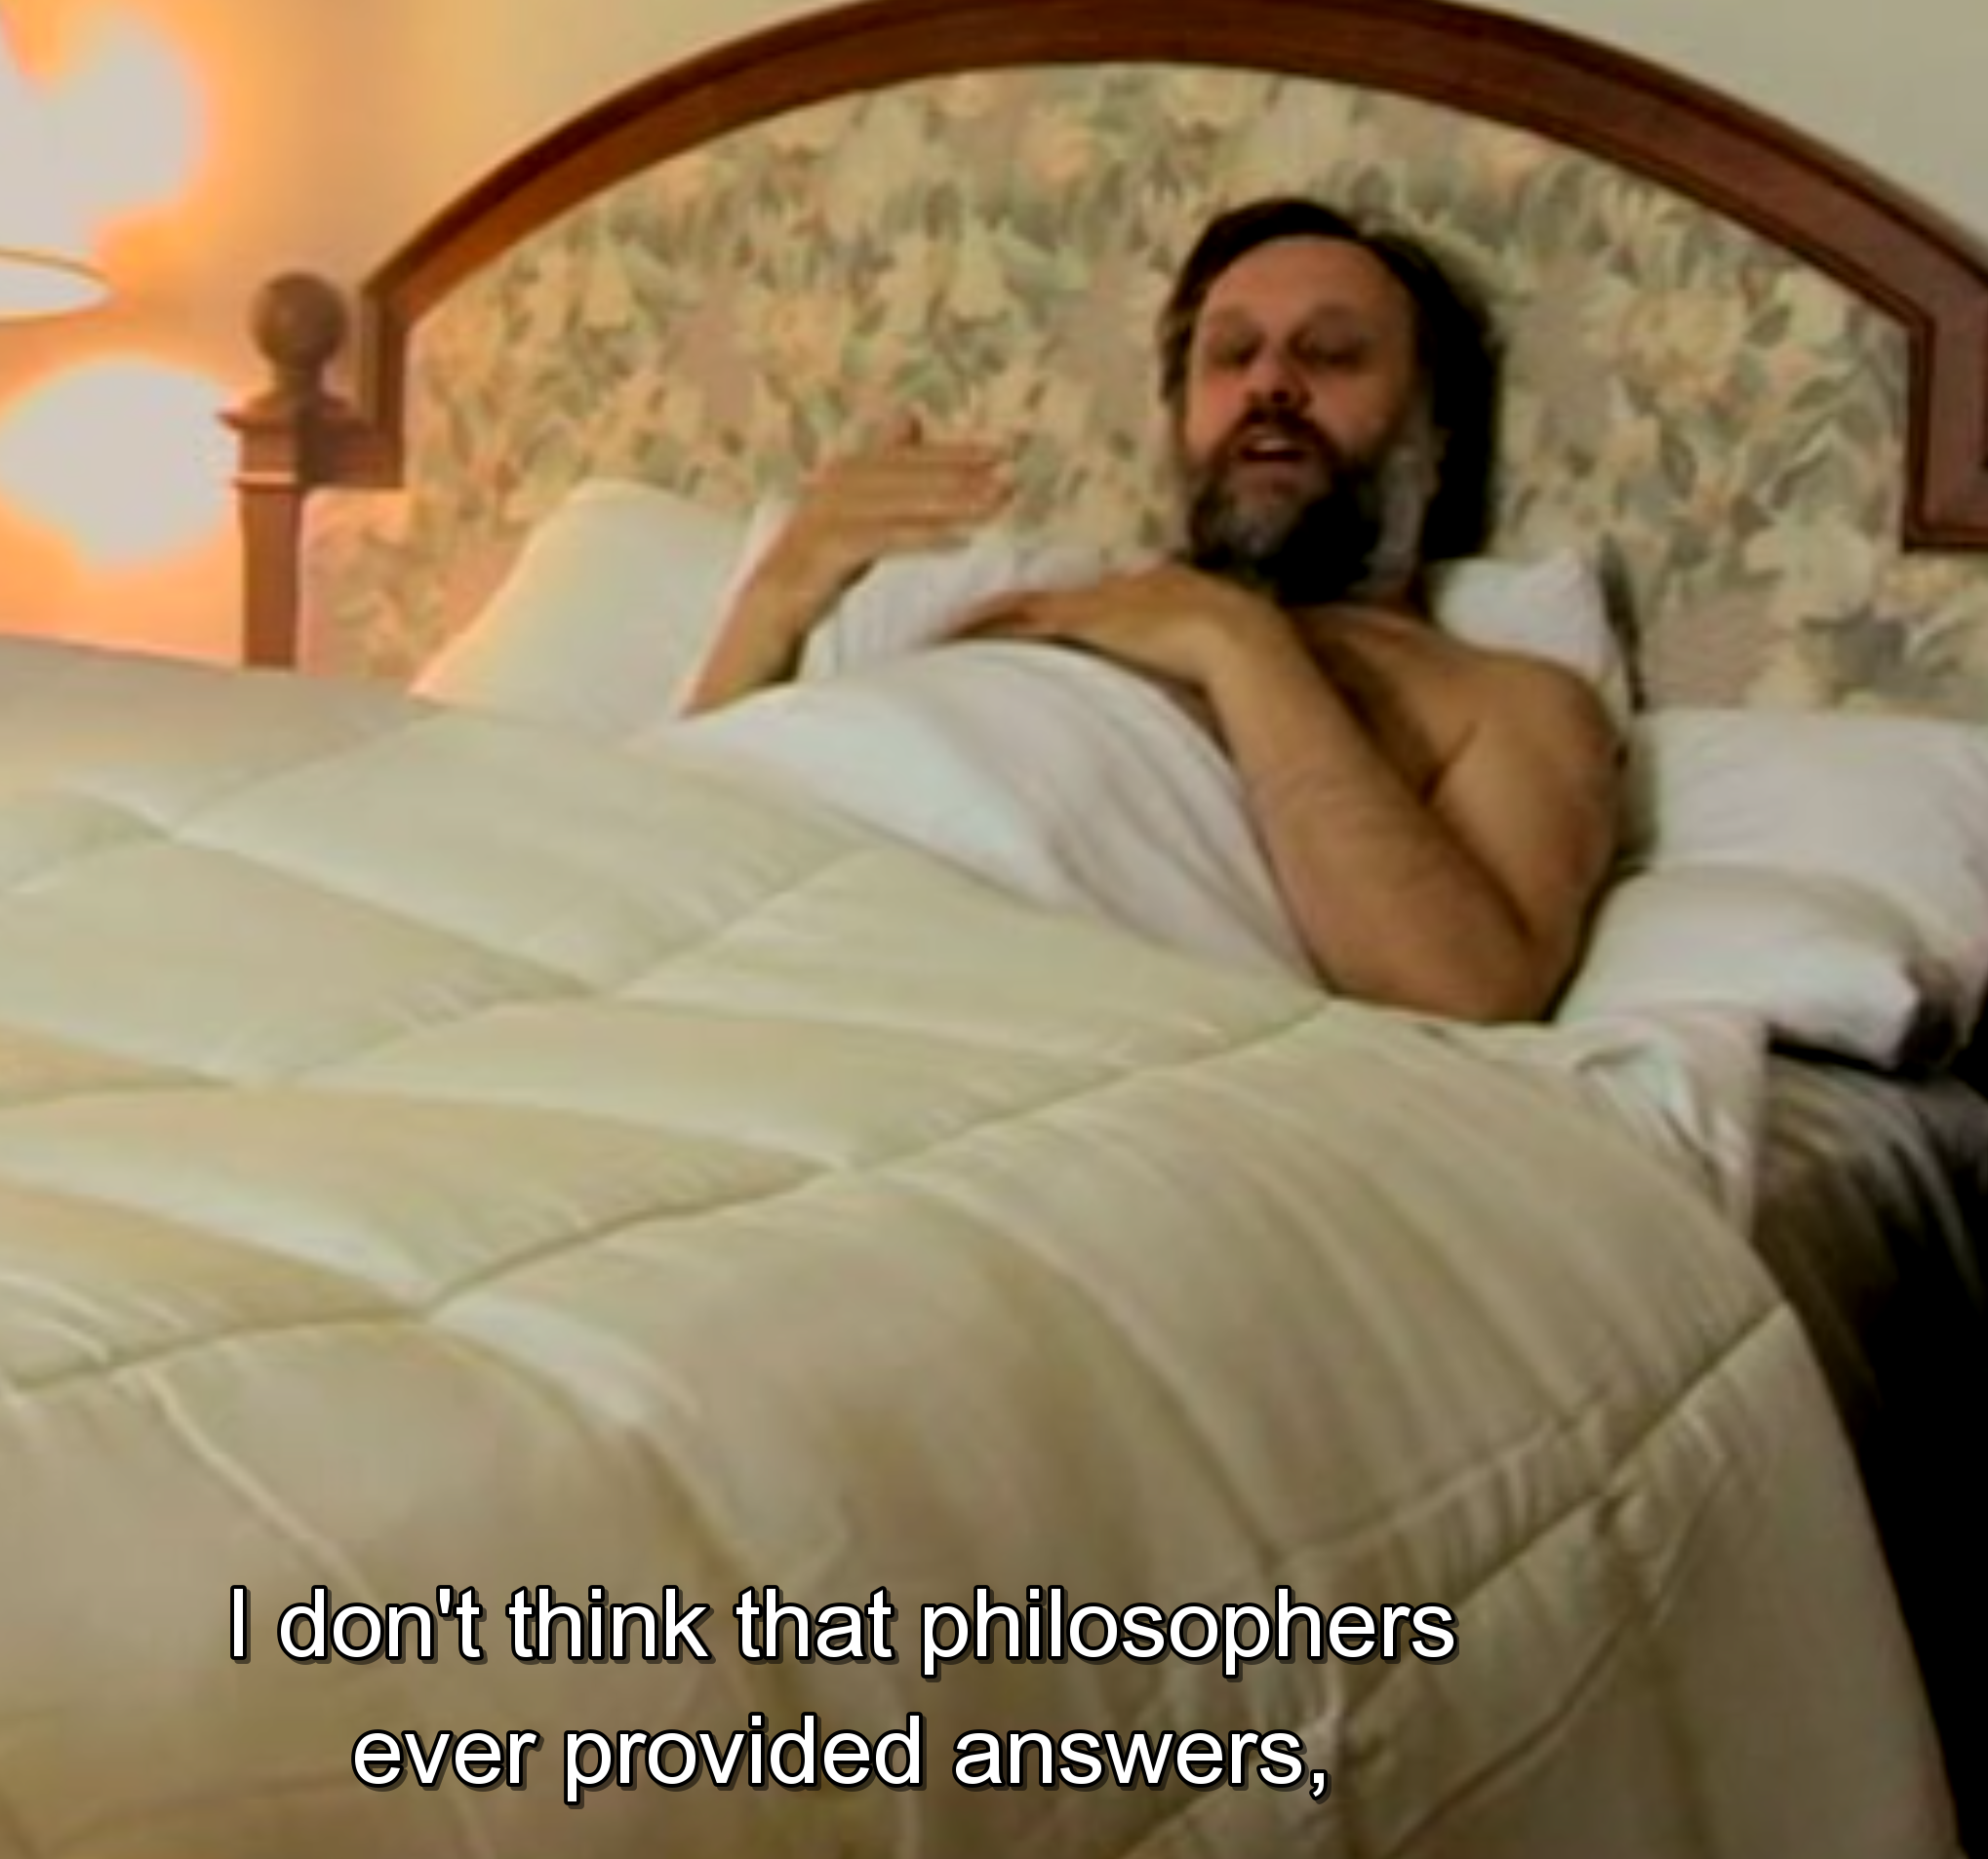
\includegraphics[width=0.5\textwidth]{images/template.png}
%	\caption{Template Bild}
%	\label{fig:template}
%\end{figure}

\end{document}
